\documentclass{beamer}
\usetheme{tokitex}

\usepackage{graphics}
\usepackage{multirow}
\usepackage{tabto}

\usepackage[english,bahasa]{babel}
\newtranslation[to=bahasa]{Section}{Bagian}
\newtranslation[to=bahasa]{Subsection}{Subbagian}

\usepackage{listings, lstautogobble}
\usepackage{color}

\definecolor{dkgreen}{rgb}{0,0.6,0}
\definecolor{gray}{rgb}{0.5,0.5,0.5}
\definecolor{mauve}{rgb}{0.58,0,0.82}

\lstset{frame=tb,
  language=pascal,
  aboveskip=1mm,
  belowskip=1mm,
  showstringspaces=false,
  columns=fullflexible,
  keepspaces=true,
  basicstyle={\small\ttfamily},
  numbers=none,
  numberstyle=\tiny\color{gray},
  keywordstyle=\color{blue},
  commentstyle=\color{dkgreen},
  stringstyle=\color{mauve},
  breaklines=true,
  breakatwhitespace=true,
  autogobble=true
}

\title{Perkenalan Graph}
\author{Tim Olimpiade Komputer Indonesia}
\date{}

\usepackage{verbatim}
\lstset{escapeinside={<@}{@>},belowskip=\baselineskip}
\definecolor{mygreen}{rgb}{0, 0.597, 0.199}

\begin{document}

\begin{frame}
\titlepage
\end{frame}

\begin{frame}
\frametitle{Pendahuluan}
Melalui dokumen ini, kalian akan:
\begin{itemize}
  \item Mengenal konsep dan terminologi graph
  \item Mengetahui jenis-jenis graph
  \item Mengenal representasi graph pada pemrograman
  \item Mengenal metode-metode yang digunakan dalam graph
\end{itemize}

\end{frame}

\begin{frame}
\frametitle{Mengenal Graph}
Graph merupakan struktur data yang terdiri dari \alert{node/vertex} dan \alert{edge}. Node direpresentasikan dengan bentuk lingkaran dan edge direpresentasikan dengan bentuk garis pada ilustrasi di bawah ini.

\begin{figure}
  \centering
  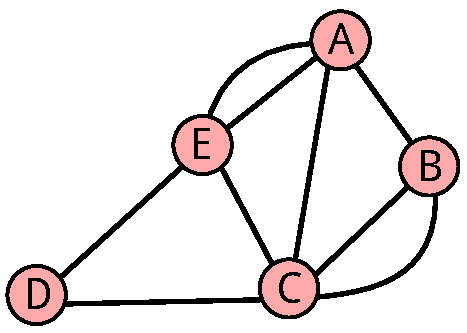
\includegraphics[width=6 cm]{asset/graph.pdf}
\end{figure}
\end{frame}

\begin{frame}
\frametitle{Mengenal Graph (lanj.)}
\begin{itemize}
  \item Edge berfungsi untuk menghubungkan antar node
  \item \alert{Degree} sebuah node merupakan jumlah edge yang terhubung pada node tersebut
  \item Pada contoh ilustrasi graph di slide sebelumnya, degree node A = 4, degree node B = 3, dan seterusnya.
  \item Tidak ada syarat khusus mengenai degree pada suatu graph.
  \item Berbeda dengan tree yang mana maksimal memiliki 2 children dan 1 parent
\end{itemize}

\end{frame}

\begin{frame}
\frametitle{Jenis-jenis Graph}
Berdasarkan hubungan antar node, graph terbagi menjadi 2:
\begin{itemize}
  \item Directed graph, yaitu graph satu arah. Pada graph jenis ini, jika terdapat edge dari A ke B, maka belum tentu terdapat edge dari B ke A. Contoh graph ini adalah kota-kota sebagai nodenya dan jalan 1 arah sebagai edgenya.
  \item Undirected graph, yaitu graph dua arah. Dalam graph ini, jika terdapat edge dari A ke B, maka pasti juga terdapat edge dari B ke A. Contoh graph jenis ini adalah kota-kota sebagai nodenya dan jalan 2 arah sebagai edgenya.
\end{itemize}
\end{frame}

\begin{frame}
\frametitle{Jenis-jenis Graph (lanj.)}
Berdasarkan bobot dari edgenya, graph juga terbagi menjadi 2:
\begin{itemize}
  \item Unweighted Graph, yaitu graph yang mana edgenya tidak memiliki value, sehingga semua edge memiliki weight 1 dan hanya bermakna bahwa memang terdapat hubungan antar node yang dihubungkannya.
  \item Weighted Graph, yaitu graph yang mana edgenya memiliki bobot yang berbeda-beda. Bobot pada edge ini seringkali berupa biaya atau jarak yang harus ditempuh jika menggunakan edge tersebut.
\end{itemize}
\end{frame}

\begin{frame}
\frametitle{Representasi Graph pada Pemrograman}

\begin{itemize}
  \item Dalam pemrograman, dibutuhkan sebuah struktur data agar data mengenai graph dapat disimpan dan diolah.
  \item Dapat direpresentasikan menggunakan 3 metode, yaitu adjacency matrix, adjacency list, dan edge list.
  \item Masing-masing representasi memiliki keuntungan dan kerugiannya masing-masing.
  \item Penggunaan representasi graph bergantung dengan masalah yang sedang dihadapi
\end{itemize}
\end{frame}

\begin{frame}
\frametitle{Adjacency Matrix}

\begin{itemize}
  \item Membutuhkan struktur data array 2 dimensi dengan ukuran N x N yang mana N merupakan banyaknya \foreignTerm{node/vertex}
  \item Seluruh elemen pada matrix diinisialisasi dengan suatu angka (misalnya angka nol)
  \item Angka nol tersebut menyatakan tidak ada edge
  \item Misal terdapat edge dari A ke B pada unweighted graph, ganti isi $matrix[A][B] = 1$
  \item Misal terdapat edge dari A ke B dengan bobot C, maka ganti isi $matrix[A][B] = C$
\end{itemize}

\end{frame}

\begin{frame}
\frametitle{Adjacency List}
\begin{itemize}
  \item Membutuhkan struktur data array of lists.
  \item Tiap list berisi keterangan mengenai edge yang terdapat dalam suatu node.
  \item Ukuran dari array merupakan N yang mana N merupakan banyaknya node/vertex
  \item Inisialisasi seluruh list kosong, yang menandakan bahwa belum terdapat edge dalam graph tersebut.
  \item Misal terdapat edge dari A ke B pada unweighted graph, maka masukkan B kedalam list A.
  \item Misal terdapat edge dari A ke B dengan bobot C, masukkan \{B,C\} kedalam list A.
\end{itemize}
\end{frame}

\begin{frame}
\frametitle{Edge List}

\begin{itemize}
  \item Membutuhkan struktur data sebuah list.
  \item Seluruh keterangan edge dimasukkan kedalam list tersebut.
  \item Berbeda dengan adjacency list yang membutuhkan array of list, pada edge list hanya dibutuhkan satu buah list.
  \item Inisialisasikan list tersebut kosong.
  \item Misal terdapat edge dari A ke B pada unweighted graph, masukkan \{A,B\} kedalam list tersebut
  \item Misal terdapat edge dari A ke B dengan bobot C, maka masukkan \{A,B,C\} kedalam list tersebut
\end{itemize}

\end{frame}


\begin{frame}[fragile]
\frametitle{Pseudocode Representasi Graph}

Adjacency Matrix
\begin{lstlisting}
  integer AdjMatrix[N][N]
  set AdjMatrix = 0
  
  <@\textcolor{mygreen}{//edge dari 1 ke 4 pada undirected unweighted graph}@>
  AdjMatrix[1][4] = 1
  AdjMatrix[4][1] = 1
\end{lstlisting}
Adjacency List
\begin{lstlisting}
  List<integer> AdjList[N]
  
  <@\textcolor{mygreen}{//edge dari 1 ke 4 pada undirected unweighted graph}@>
  AdjList[1].push(4)
  AdjList[4].push(1)
  
\end{lstlisting}
\end{frame}

\begin{frame}[fragile]
\frametitle{Pseudocode Representasi Graph (lanj.)}

Edge List
\begin{lstlisting}
  List<{integer,integer}> EdgeList
  
  <@\textcolor{mygreen}{//edge dari 1 ke 4 pada undirected unweighted graph}@>
  EdgeList.push({1,4})
  
  List<{integer,integer,integer}> WeightedList
  
  <@\textcolor{mygreen}{//edge dari 2 ke 3 dengan bobot 5 pada undirected graph}@>
  WeightedList.push({2,3,5})
\end{lstlisting}
\end{frame}

\begin{frame}
\frametitle{Keuntungan dan Kerugian Representasi Graph}
Misalkan graph kita memiliki V vertex dan E edge. Kita ingin melihat kompleksitas yang dibutuhkan berbagai jenis representasi graph pada suatu node yang mana node tersebut memiliki jumlah tetangga sebanyak K.
{\fontsize{9}{10}\selectfont\renewcommand{\arraystretch}{1.75}
\begin{center}
 \begin{tabular}{||c|c c c c||} 
 \hline
 Representasi & TambahEdge & HapusEdge & DaftarTetangga & CekHubungan \\ [0.5ex] 
 \hline\hline
 Adj.Matrix & konstan & konstan & N & konstan\\ 
 \hline
 Adj.List & konstan & K & K & K\\
 \hline
 Edge List & konstan & E & E & E\\
 \hline
\end{tabular}
\end{center}
}
Tabel di atas menjelaskan kompleksitas yang dibutuhkan untuk melakukan proses-proses dalam graph
\end{frame}

\begin{comment}
\begin{frame}
\frametitle{Keuntungan dan Kerugian Representasi Graph}

\begin{itemize}
  \item Adjacency Matrix memakan lebih banyak memori. Hal ini dikarenakan adjacency matrix menyimpan keterangan dari satu node ke semua node. Sedangkan dalam adjacency list, suatu node hanya menyimpan keterangan mengenai node lain yang memiliki edge. Oleh karena itu, adjacency list lebih baik digunakan ketika edge yang terdapat tidak teralu banyak.
  \item Untuk melakukan pengecekan atau perubahan edge dari A ke B, pada adjacency matrix dapat dilakukan dengan hanya melihat dan mengubah matrix[A][B]. Sedangkan pada adjacency list, kita harus mengiterasi seluruh elemen pada list[A]
\end{itemize}
\end{frame}

\begin{frame}
\frametitle{Keuntungan dan Kerugian Representasi Graph (lanj.)}
\begin{itemize}
  \item Jika ada edge dari A ke B yang akan dibuang, maka pada adjacency matrix kita hanya perlu mengubah nilai Matrix[A][B]. Sedangkan pada adjacency list, harus dilakukan iterasi terlebih dahulu untuk mencari edge tersebut, lalu menghapusnya juga lebih rumit karena harus menggeser seluruh elemen setelahnya.
  \item Untuk mencari tetangga-tetangganya, maka pada adjacency matrix perlu dilakukan iterasi terhadap seluruh node yagn ada. Sementara itu, pada adjacency list hanya perlu dilakukan iterasi pada list yang isinya merupakan tetangga dari node yang bersangkutan.
\end{itemize}
\end{frame}
\end{comment}

\begin{frame}
\frametitle{Graph Traversal}

\begin{itemize}
  \item Representasi Graph saja belum berguna karena belum dapat mencari informasi mengenai suatu graph
  \item \alert{Graph Traversal} merupakan penelusuran node-node pada suatu graph.
  \item Contoh permasalahannya adalah diberikan node A dan node B, ditanya apakah dari node A bisa pergi ke node B menggunakan edge yang ada?
  \item Permasalahan tersebut dapat diselesaikan menggunakan graph traversal.
  \item Terdapat 2 metode yang dapat digunakan, yaitu DFS dan BFS.
\end{itemize}
\end{frame}

\begin{frame}
\frametitle{DFS}

\alert{DFS} merupakan singkatan dari Depth-First Search. Berdasarkan namanya, dapat disimpulkan bahwa DFS akan mencari node-node yang lebih dalam(depth-first) terlebih dahulu. Sebagai contoh misal terdapat graph seperti berikut

\begin{figure}
  \centering
  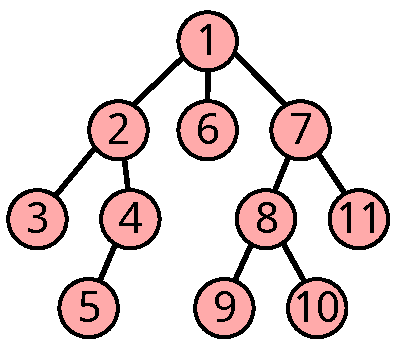
\includegraphics[width=5 cm]{asset/dfs.pdf}
\end{figure}
\end{frame}

\begin{frame}
\frametitle{DFS (lanj.)}
\begin{itemize}
  \item Angka pada gambar di atas menunjukkan urutan node tersebut dikunjungi. (Node 1 dikunjungi pertama, node 2 dikunjungi kedua, dan seterusnya)
  \item Dari urutan pengunjungan node pada gambar, dapat dililhat bahwa DFS akan mencoba menelusuri node-node yang dalam terlebih dahulu
  \item Node yang dekat dengan node awal (seperti node 7 dan 8) akan dikunjungi setelah DFS selesai mengunjungi node yang lebih dalam (seperti node 3,4, dan 5)
  \item Dalam pemrograman, DFS dapat dilakukan menggunakan rekursi atau dengan bantuan struktur data \foreignTerm{stack}
\end{itemize}
\end{frame}

\begin{frame}
\frametitle{BFS}

\alert{BFS} merupakan singkatan dari Breadth-First Search. Berdasarkan namanya, dapat disimpulkan bahwa BFS akan menelusuri node pada graph sesuai dengan layernya. Semakin dekat dengan node awal, maka node tersebut akan dikunjungi terlebih dahulu. Begitu pula sebaliknya. Sebagai contoh misal terdapat graph seperti berikut

\begin{figure}
  \centering
  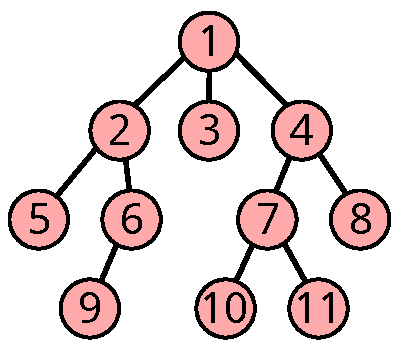
\includegraphics[width=5 cm]{asset/bfs.pdf}
\end{figure}

\end{frame}

\begin{frame}
\frametitle{BFS (lanj.)}
\begin{itemize}
  \item Angka pada gambar di atas menunjukkan urutan node tersebut dikunjungi. (Node 1 dikunjungi pertama, node 2 dikunjungi kedua, dan seterusnya)
  \item Dapat disimpulkan bahwa BFS akan mencoba mengunjungi node-node yang lebih dekat dengan node awal terlebih dahulu.
  \item Node yang jauh dengan node awal akan dikunjungi terakhir.
  \item Dalam pemrograman, BFS dapat dilakukan menggunakan bantuan struktur data \foreignTerm{queue}
  \item Slide selanjutnya akan menjelaskan implementasi DFS dan BFS pada unweighted graph yang direpresentasikan menggunakan adjacency matrix
\end{itemize}
\end{frame}

\begin{frame}[fragile]
\frametitle{Implementasi DFS}
DFS dapat diimplementasikan menggunakan rekursi atau dengan bantuan struktur data stack. Berikut adalah implementasi DFS rekursi\newline
\begin{lstlisting}
integer AdjMatrix[N][N]
boolean flag[N]
set flag = false
flag[1] = true

procedure DFS(integer currNode):
  for i=1 to N
    <@\textcolor{mygreen}{//check apakah ada edge dan belum pernah dikunjungi}@>
    if AdjMatrix[currNode][i]==1 and flag[i]==false
      flag[i] = true
      DFS(i)
end
        
\end{lstlisting}
\end{frame}

\begin{frame}[fragile]
\frametitle{Implementasi DFS (lanj.)}
Berikut adalah potongan kode untuk implementasi DFS menggunakan stack\newline
\begin{lstlisting}
integer AdjMatrix[N][N]
boolean flag[N]
set flag = false
stack <integer> s

s.push(1), flag[1] = true
while s is not empty
  integer currNode = s.top()
  s.pop()
  for i=1 to N
    if AdjMatrix[currNode][i]==1 and flag[i]==false
      flag[i] = true
      s.push(i)
        
\end{lstlisting}
\end{frame}

\begin{frame}[fragile]
\frametitle{Implementasi BFS}
BFS membutuhkan bantuan struktur data queue. Berikut adalah potongan kodenya\newline
\begin{lstlisting}
integer AdjMatrix[N][N]
boolean flag[N]
set flag = false
queue <integer> q

q.push(1), flag[1] = true
while q is not empty
  integer currNode = q.front()
  q.pop()
  for i=1 to N
    if AdjMatrix[currNode][i]==1 and flag[i]==false
      flag[i] = true
      q.push(i)
        
\end{lstlisting}
\end{frame}

\begin{frame}
\frametitle{Contoh Permasalahan}
Pak Dengklek tinggal di kota A. Suatu hari, beliau ingin pergi ke kota B. Terdapat beberapa jalan yang menghubungkan kota-kota dalam negara tempat beliau tinggal. Namun, karena beliau sudah tua, Pak Dengklek ingin melewati jalan seminimal mungkin untuk sampai ke kota B.
\newline\newline
Diberikan keterangan mengenai kota A, kota B, dan jalan-jalan yang terdapat dalam negara Pak Dengklek, outputkan berapa jalan minimal yang beliau harus lewati untuk pergi dari kota A ke kota B!
\end{frame}

\begin{frame}
\frametitle{Pembahasan Permasalahan}
Permasalahan di atas dapat diselesaikan menggunakan BFS. Karena sifat BFS yang menelusuri node per layer, maka dapat disimpulkan bahwa jika suatu node terkunjungi, maka pasti jarak yang ditempuh merupakan jarak terpendek dari node awal. Hal ini berlaku pada unweighted graph yang edgenya tidak memiliki bobot.
\newline\newline
Dengan demikian, permasalahan di atas dapat diselesaikan dengan menggunakan BFS. Pada slide selanjutnya akan diberikan contoh implementasi untuk menyelesaikan permasalahan jarak terpendek tersebut!
\end{frame}

\begin{frame}[fragile]
\frametitle{Implementasi Permasalahan}

\begin{lstlisting}
integer AdjMatrix[N][N] , A , B , jarak = -1
queue < (integer,integer) > q
<@\textcolor{mygreen}{//Queue menyimpan node yang dikunjungi dan jarak dari A}@>
q.push({A,0}), flag[A] = true
while q is not empty
  (integer,integer) currNode = q.front()
  q.pop()
  <@\textcolor{mygreen}{//Cek jika telah sampai di kota B}@>
  if currNode.first == B
    jarak = currNode.second, break
  for i=1 to N
    if AdjMatrix[currNode.first][i]==1 and flag[i]==false
      flag[i] = true
      q.push({i,currNode.second+1})
if jarak!=-1
  print jarak
else
  print 'Tidak dapat ke kota B'    
\end{lstlisting}
\end{frame}

\begin{frame}
\frametitle{Tree}
\begin{itemize}
  \item \foreignTerm{Tree} merupakan bentuk khusus dari graph
  \item Seluruh node pada tree terhubung (tidak ada node yang tidak dapat dikunjungi dari node lain) dan tidak terdapat \alert{cycle}
  \item Jumlah edge dalam sebuah tree pasti berjumlah sebanyak (Node - 1)
\end{itemize}

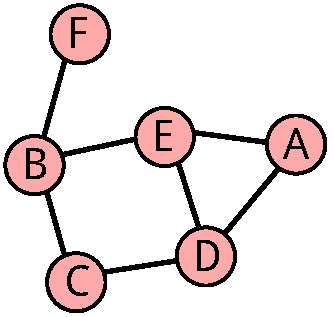
\includegraphics[width=3.5 cm]{asset/not-tree.pdf}
\hspace{\fill}
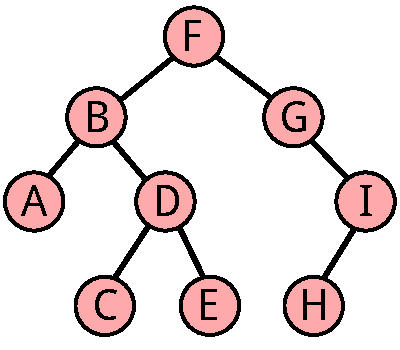
\includegraphics[width=4 cm]{asset/tree.pdf}
\newline\newline
Pada gambar di atas, gambar kiri bukan sebuah tree karena memiliki cycle, sedangkan gambar kanan merupakan tree. 
\end{frame}

\begin{frame}
\frametitle{Directed Acyclic Graph}
\begin{itemize}
  \item \foreignTerm{Directed Acyclic Graph (DAG)} merupakan bentuk khusus dari directed graph.
  \item DAG tidak memiliki \alert{direct cycle}
  \item Berbeda dengan tree yang mana setiap nodenya harus dapat dicapai node lainnya, sifat tersebut tidak berlaku pada DAG
\end{itemize}

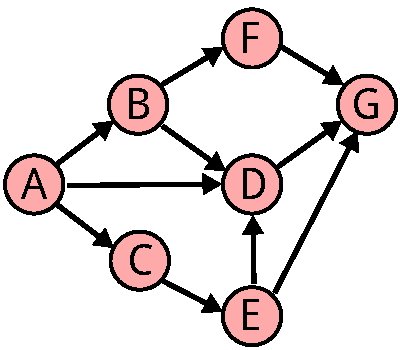
\includegraphics[width=4 cm]{asset/dag.pdf}
\hspace{\fill}
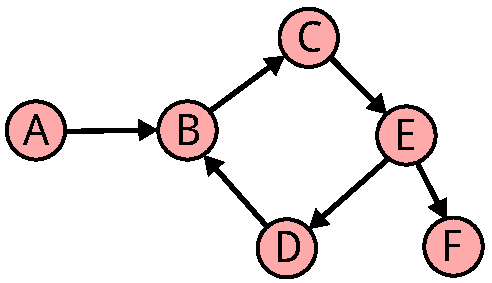
\includegraphics[width=5 cm]{asset/not-dag.pdf}
\newline\newline
Pada gambar di atas, gambar kiri merupakan DAG, sedangkan gambar kanan bukan DAG karena memiliki cycle
\end{frame}

\end{document}
